The parallel implementation for PFEM-2 follows the guidelines presnted in \cite{gimenez:parallel} for the case of distributed memory architectures. The challenges are well described in their paper but basically involves the extra amount of memory needed for the particle data structure. Due to the explicit scheme the parallel implementation needs to take care of local operations to each particle separately from the rest allowing for trivial parallelization. The dificulty arise at the interface between processors where particles may travel several elements and possible processors before finding their final host element. This task requieres an outer loop to communicate particles that will terminate when no more particles cross the interface between partitions. In figure \ref{fig:parallel} there is an illustration of how particles may move across processors. The thick black line depicts the partition. In the first case a particle lands in the same processor which involves no communication. In the second case a particle moves across a single interface and communication takes place. In the third place a particle may move accross two or more processors in which case the outer loop will perform as many communications as necessary untill no more particles cross a processor interface.

\begin{figure}[htp] 
\centering 
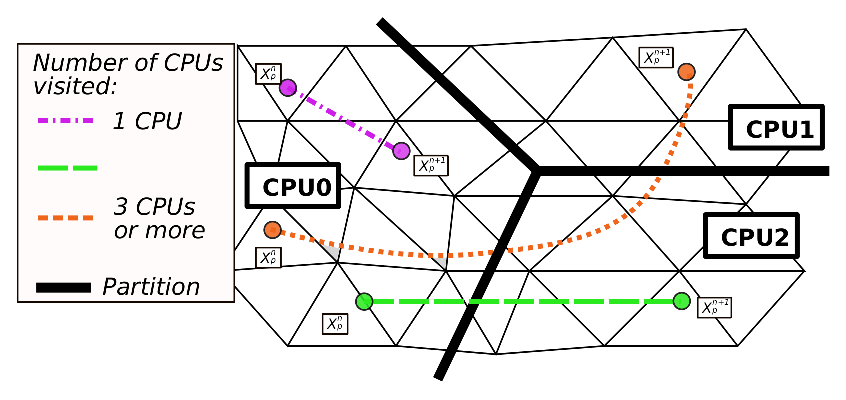
\includegraphics[scale=.6]{./imgs/parallel.eps}
\caption{Different ways that particles may move across processor interfaces.}
\label{fig:parallel}
\end{figure}


The current approach is built ``on top'' of a pre-existing parallel FEM implementation thus inheriting much of the data structures and methodologies. The partitions are creating using the software METIS \cite{metis1,metis}...

In the present implementation load balancing has not being addressed. Strictly speaking if particles are not removed at some point accumulation of particles in one partition will be an issue. Most luckily the PFEM-2 impliementation will change to allow removal of particles in such a way that an almost constant amount of particles is preserved for each element. The techniques for particle inventory presented in \cite{gimenez-difusion} will be a good starting point for the implementation.

To exemplify scalability a $3-d$ problem of the flow past a cylinder is used. It has a relatively small number of elements of about 200K compared to the element numbers used in the application examples. 
In figure \ref{fig:scalab} the strong scalability of the full formulation (FEM+PFEM-2) is shown for shared memory parallelization. There are two curves for two different inventory strategies. In the first case the number of particles is kept constant at each element. The total number of particles in this case is around 5.7M. In the second case the number of particles changes. No particle is removed from the model except for those that leave the domain and particles are added in elements with less than 12 particles. So the total number of particles is expected to increase. The final number reaches about 30M particles. Since there is no load balancing particles that accumulate in an element are expected to degrade the scalability which is what is obsreved in \ref{fig:scalab}. The total scalability compares well with that of \cite{gimenez:parallel}.

\begin{figure}[htp] 
\centering 
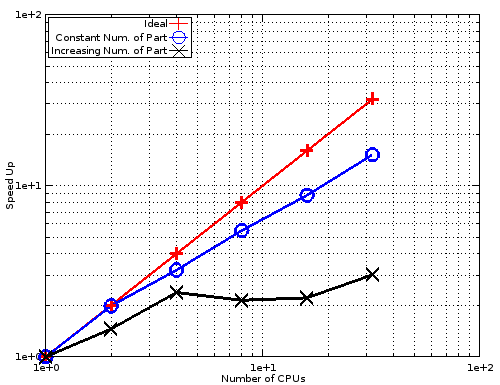
\includegraphics[scale=.6]{./imgs/scalability1.png}
\caption{Scalability plot for the cases where the number of particles per element is kept constant and the case where no particle removal takes place so the number of particles increase without load balancing.}
\label{fig:scalab}
\end{figure}


 
